% ============================================================
% SQLAS + NexusSQL — IEEE ICDE 2027 Industrial & Applications Track
% Compiler: pdfLaTeX
% All results tables are generated by bench/make_paper_tables.py and
% included from paper_tables/ — do not hand-edit numbers here.
% ============================================================
\documentclass[conference]{IEEEtran}

% ── Packages ─────────────────────────────────────────────────
\usepackage[T1]{fontenc}
\usepackage[utf8]{inputenc}
\usepackage{amsmath,amssymb}
\usepackage{graphicx}
\usepackage{booktabs}
\usepackage{multirow}
\usepackage{xcolor}
\usepackage{url}
\usepackage{microtype}
\usepackage{listings}
\usepackage{array}
\usepackage{tabularx}
\usepackage{tikz}
\usepackage{pgfplots}
\pgfplotsset{compat=1.18}
\usetikzlibrary{shapes.geometric,arrows.meta,positioning,fit,backgrounds,calc}
% pgf-pie removed — verdict figure uses xbar stacked, not pie

% ── Custom TikZ styles ───────────────────────────────────────
\tikzset{
  box/.style={rectangle,rounded corners=3pt,draw=#1,fill=#1!12,
    minimum width=1.8cm,minimum height=0.55cm,font=\scriptsize\bfseries,
    text=black,align=center},
  arrow/.style={-{Stealth[length=4pt]},thick,#1},
  layer/.style={rectangle,rounded corners=4pt,draw=gray!40,
    fill=gray!6,minimum width=3.8cm,minimum height=0.5cm,
    font=\scriptsize,align=center},
}
\usepackage{balance}           % balance last-page columns
\usepackage[hidelinks]{hyperref}

\lstset{
  basicstyle=\footnotesize\ttfamily,
  breaklines=true,
  frame=single,
  xleftmargin=1em,
  xrightmargin=1em,
  aboveskip=4pt,
  belowskip=4pt,
}

% ── Placeholders for the in-progress human annotation study ──
% (values inserted in the camera-ready once annotation completes)
\newcommand{\humanKappa}{\textit{pending}}
\newcommand{\humanRho}{\textit{pending}}

% ── Title ─────────────────────────────────────────────────────
\title{SQLAS: A Multi-Dimensional Evaluation Framework and Large-Schema
Benchmark for SQL Agents, with a Production Case Study}

\author{
  \IEEEauthorblockN{Pradip Tivhale}
  \IEEEauthorblockA{Independent Researcher\\
    Email: pradiptivhale@gmail.com}
}

\begin{document}

\maketitle

% ── Abstract ─────────────────────────────────────────────────
\begin{abstract}
Enterprise databases routinely contain hundreds of tables, yet SQL-agent
evaluation remains anchored to small-schema academic benchmarks (Spider:
avg.\ 5.3 tables/DB) and to a single binary metric --- execution accuracy
--- that ignores safety, output quality, and upstream schema retrieval.
We present \textbf{SQLAS}, an evaluation framework designed specifically
for SQL agents: a three-dimension AND-logic verdict (correctness /
quality / safety), a zero-LLM-call safety suite (AST-based read-only
enforcement, SQL/prompt-injection and PII detectors), a schema-retrieval
F1 metric for upstream table selection, and a 15-category failure
taxonomy with remediation hints. We accompany the framework with
\textbf{LargeSchemaEval}, an open benchmark of merged Spider databases
at 50/100/200/500-table scale points with AST-repaired gold SQL, and
with \textbf{NexusSQL}, a production full-stack SQL agent reported as a
case study.

Applying SQLAS end to end yields deliberately honest findings. On the
full BIRD dev set (1{,}534 questions, zero-shot, manifest-pinned),
NexusSQL reaches \textbf{62.3\%} execution match (Wilson 95\% CI
[59.8, 64.6]; VES 0.700). A two-scale ablation of four schema-retrieval
modes at 105 and 502 tables finds all modes \emph{statistically
indistinguishable} (McNemar $p = 0.58$--$1.0$): retrieval-based schema
linking is a \emph{cost} optimization --- cutting prompt tokens by
95.3\% at 200 tables --- not an accuracy mechanism, and full-schema
injection remains more accurate wherever the schema fits the context
window. A 100-query LLM-judged evaluation yields a \textbf{76.0\%} PASS
rate under the three-dimension verdict, and every query in the reported
campaigns passed the AST-based read-only safety check.
\end{abstract}

\noindent\textit{Code and benchmark:} \url{https://github.com/thepradip/NexusSQL}

\begin{IEEEkeywords}
Text-to-SQL, SQL agent, schema retrieval, LLM evaluation, enterprise database, large-schema, BIRD benchmark
\end{IEEEkeywords}

% ──────────────────────────────────────────────────────────────
\section{Introduction}
\label{sec:intro}
% ──────────────────────────────────────────────────────────────

\subsection{The Enterprise SQL Problem}

Modern enterprise databases are orders of magnitude larger than academic
benchmarks assume. SAP S/4HANA deployments routinely contain 2,000+
tables; Oracle EBS 1,500+; Salesforce 800+. Yet Spider~\cite{spider},
the dominant Text-to-SQL benchmark, has an average of 5.3 tables per
database. BIRD~\cite{bird}, its harder successor, reaches only 37 tables.
Systems trained and evaluated on these benchmarks face a fundamental
scalability problem in enterprise settings.

The problem manifests as \emph{context explosion}. A naive full-schema
injection approach at 200 tables requires approximately 41,300 tokens per
query, just for the schema context. At 1,000 queries per day with
GPT-4o pricing, this translates to $\approx$\$75,000/year. More
critically, as schema size approaches the LLM's effective context
window, SQL generation quality degrades due to the
``lost-in-the-middle'' effect~\cite{lostmiddle}; the model attends
poorly to relevant tables buried in a long schema dump.

\textbf{A concrete motivating example.}
Consider a business analyst at a mid-size manufacturer who types:
\emph{``Which customers had the highest revenue last quarter?''}
The underlying ERP database has 200 tables spanning procurement,
logistics, HR, and finance. A naive full-schema injection approach
sends all 200 table definitions to the LLM in a single prompt --- consuming
41,300 tokens and costing \$0.21 per query. Worse, empirical results
from LLM long-context studies~\cite{lostmiddle} show that relevant
tables buried past position 50 in a schema dump are effectively ignored,
causing the model to hallucinate column names from irrelevant tables.

NexusSQL handles this query by first running BM25 sparse retrieval over
the schema index, identifying \texttt{sales\_orders}, \texttt{customers},
and \texttt{revenue\_summary} as candidates. FK-graph expansion adds
\texttt{customer\_regions} as a JOIN partner. The end-to-end query
completes in roughly six seconds (median 5.5--6.0\,s in our 105-table
campaign) using only \textbf{1,932} prompt tokens --- a 21$\times$
reduction --- and generates SQL grounded in the inspected schema.
We emphasise up front what this retrieval does and does not buy:
our two-scale ablation (Section~\ref{sec:experiments}) shows that
retrieval-based schema linking is a \emph{cost} optimization, not an
accuracy mechanism --- retrieval modes are statistically tied at both
105 and 502 tables, and full-schema injection is more accurate wherever
the schema fits the context window.

\textbf{Why existing systems fail at enterprise scale.}
DIN-SQL~\cite{dinsql}, CHESS~\cite{chess}, and DAIL-SQL~\cite{dailsql}
are the leading Text-to-SQL systems on BIRD and Spider leaderboards.
All three share a critical architectural assumption: the complete
database schema fits within a single LLM context window. CHESS applies
schema pruning, but its pruning operates over the full schema in a
single-pass prompt that itself requires the full schema as input.
DIN-SQL's decomposed prompting strategy uses a ``\emph{schema linking}''
step that likewise requires all table and column definitions visible
simultaneously. At 37 tables (BIRD's maximum), this assumption holds.
At 200 tables with $\approx$200 columns each, the schema alone requires
41,300 tokens --- leaving almost no room for question, few-shot examples,
or chain-of-thought reasoning within a 128K context window. At 500+
tables, full-schema injection exceeds the context limit entirely and
the system cannot produce any output. NexusSQL's adaptive retrieval
architecture is explicitly designed to break this assumption: it selects
a small set of tables (typically one to eight), making schema size
largely irrelevant to prompt length.

\subsection{The SQL Agent Evaluation Gap}

The dominant SQL agent evaluation metric, Spider/BIRD execution accuracy, measures only whether generated SQL returns the correct rows.
It leaves critical production questions unanswered:
\begin{itemize}
  \item Did schema retrieval select the right tables? (upstream quality)
  \item Is the SQL well-formed, efficient, and schema-compliant? (output quality)
  \item Is the query safe to execute on production data? (safety)
  \item Why did it fail, and what should be fixed? (actionable feedback)
\end{itemize}

To illustrate the evaluation gap concretely, consider a query on an HR
database: \emph{``List all employees in the engineering department.''}
An agent generates \texttt{SELECT name, ssn, salary FROM employees WHERE
dept = `Engineering'} --- which returns the correct rows (execution
accuracy = 1.0) but exposes SSN values of every employee. Under
Spider/BIRD evaluation, this query is graded \textbf{PASS}.
Under SQLAS evaluation, the PII access detector flags the \texttt{ssn}
column and issues a \texttt{FAIL\_SAFETY} verdict with a safety score
of 0.0, overriding the perfect execution accuracy. This distinction
between ``gets the right rows'' and ``is safe to run in production''
is precisely the gap SQLAS addresses.

SQLAS addresses this gap with a multi-dimension evaluation framework
designed specifically for SQL agents, covering correctness, quality,
safety, and upstream schema retrieval in a single verdict.

\subsection{Contributions}

\begin{enumerate}
  \item \textbf{SQLAS}: a multi-dimension evaluation framework built
        specifically for SQL agents --- a three-dimension AND-logic verdict
        (correctness / quality / safety), a zero-LLM-call safety suite,
        a schema-retrieval F1 metric for upstream table selection, and a
        15-category failure taxonomy with actionable remediation hints.
  \item \textbf{LargeSchemaEval}: an open benchmark of merged Spider
        databases at 50/100/200/500-table scale points (up to 502
        tables), with AST-repaired gold SQL.
  \item \textbf{A two-scale retrieval ablation} showing that four
        schema-retrieval modes are statistically indistinguishable in
        execution match at both 105 and 502 tables: retrieval-based
        schema linking is a cost optimization (95.3\% prompt-token
        reduction at 200 tables), not an accuracy mechanism.
  \item \textbf{NexusSQL}: a production full-stack SQL agent (four-layer
        adaptive retrieval, forced-plan ReAct loop, AST-based safety
        enforcement), reported as a case study with deployment lessons.
  \item \textbf{An evaluation-integrity methodology}: per-row
        retrieval-mode provenance, manifest-pinned benchmark runs,
        error-driven gold-set repair, and a full re-run that replaced
        all earlier numbers.
\end{enumerate}

Figure~\ref{fig:arch_overview} provides a complete overview of the NexusSQL system
and the SQLAS evaluation framework, showing how both components interact
across the full query lifecycle.

% ── Full-width overview figure (spans both columns) ───────────
\begin{figure*}[!t]
\centering
\includegraphics[width=0.98\textwidth]{nexussql_architecture.png}
\caption{NexusSQL system architecture. The 4-layer adaptive retrieval pipeline
(L1: BM25 Sparse $\to$ L2: Dense Embeddings $\to$ L3: RRF Fusion $\to$
L4: FK-Graph + Adaptive Threshold) selects an average of 2.16 tables from
100+ table schemas, reducing prompt tokens by 95.3\% versus full-schema injection.
Simple queries take the Fast Pipeline (1 LLM call); complex queries use the
ReAct Agent with a mandatory forced-plan step. SQLAS provides end-to-end evaluation
across correctness, quality, and safety dimensions with AND-logic verdict.}
\label{fig:arch_overview}
\end{figure*}

% ──────────────────────────────────────────────────────────────
\section{Related Work}
\label{sec:related}
% ──────────────────────────────────────────────────────────────

\subsection{Text-to-SQL Systems}

Recent LLM-based approaches have improved accuracy on standard
benchmarks through decomposed generation~\cite{dinsql}, structured
prompt selection~\cite{dailsql}, and schema filtering~\cite{chess}.
However, these systems are evaluated exclusively on Spider and BIRD,
where individual databases contain at most 37 tables. Their reliance
on full-schema injection makes them impractical for enterprise databases
with hundreds of tables, a gap NexusSQL directly addresses.

\subsection{Schema Linking Approaches}

A parallel line of research focuses on schema linking --- the task of
identifying which tables and columns a question requires before SQL
generation. RAT-SQL~\cite{ratsql} introduced relation-aware schema
encoding with a graph neural network that explicitly models question-schema
alignments, achieving strong results on Spider by linking question tokens
to relevant column nodes. ShadowGNN~\cite{shadowgnn} extended this with
graph projection networks that capture cross-database structural patterns.
SADGA (Structure-Aware Dual Graph Aggregation~\cite{sadga}) further
models the dual graph between question and schema.

These approaches advance schema linking accuracy on Spider (up to 37
tables) and BIRD (up to 37 tables), but share a fundamental limitation
in enterprise contexts: they require the \emph{full schema graph} as
input to the GNN encoder. At 100+ tables, the graph computation becomes
a quadratic bottleneck, and none of these systems have been evaluated
beyond 37-table databases. Furthermore, they are trained end-to-end on
Spider/BIRD schema distributions and do not include production features
such as multi-tenant access control, PII detection, or read-only
enforcement. NexusSQL's retrieval-first architecture sidesteps the full
graph encoding requirement by reducing the candidate schema to 2--8
tables before any LLM or GNN processing.

\subsection{Enterprise SQL and RAG-Based Systems}

DB-GPT~\cite{dbgpt} is an open-source Text-to-SQL system that uses
retrieval-augmented generation to ground SQL generation in schema
context. WrenAI is a commercial Text-to-SQL assistant that applies
semantic layer caching to reduce redundant LLM calls. Both systems
represent the RAG-based paradigm: retrieve relevant schema fragments,
inject into an LLM prompt, generate SQL. However, neither system
provides systematic evaluation beyond execution accuracy: there is no
schema retrieval F1 metric, no multi-dimension safety verdict, and no
structured failure taxonomy. SQLAS fills this evaluation gap for both
NexusSQL and, in principle, any SQL agent including DB-GPT and WrenAI.

\subsection{LLM and SQL Evaluation Frameworks}

Table~\ref{tab:ragas_comparison} compares SQLAS against existing evaluation
frameworks. RAGAS~\cite{ragas} targets retrieval-augmented generation pipelines
and covers faithfulness and answer relevance, but has no support for SQL
execution, schema validation, or safety checks. ARES~\cite{ares} and
TruLens~\cite{trulens} provide general LLM observability with no
SQL-specific metrics.

The closest prior work is STEF~\cite{stef}, a concurrent SQL evaluation
framework designed for production monitoring without access to ground-truth
SQL or database schema. STEF is \emph{schema-agnostic} by design, scoring
queries from natural language alone. SQLAS takes a complementary approach:
it operates with database access and gold SQL to compute execution accuracy,
schema retrieval F1, and safety checks that STEF does not measure.
To illustrate the distinction concretely: given the question
\emph{``How many orders were placed last month?''} and the generated SQL
\texttt{SELECT COUNT(*) FROM orders WHERE date >= \ldots},
STEF can assess whether the natural language answer is coherent and
relevant, but cannot verify that (a) the \texttt{orders} table was
correctly retrieved from a 200-table schema, (b) the SQL will actually
execute and return the correct count, or (c) the query does not scan a
PII-adjacent table. SQLAS measures all three.
The two frameworks serve different deployment contexts: STEF for
schema-free monitoring, SQLAS for rigorous benchmarking with ground truth.

\begin{table}[!htb]
\caption{SQLAS vs General LLM Evaluation Frameworks}
\label{tab:ragas_comparison}
\centering
\small
\begin{tabular}{lcccc}
\toprule
\textbf{Capability} & \textbf{RAGAS} & \textbf{ARES} & \textbf{TruLens} & \textbf{SQLAS} \\
\midrule
Faithfulness          & \checkmark & \checkmark & \checkmark & \checkmark \\
Answer relevance      & \checkmark & \checkmark & \checkmark & \checkmark \\
SQL execution acc.    & ---        & ---        & ---        & \checkmark \\
Schema retrieval F1   & ---        & ---        & ---        & \checkmark \\
SQL injection detect. & ---        & ---        & ---        & \checkmark \\
Read-only compliance  & ---        & ---        & ---        & \checkmark \\
Failure classification& ---        & ---        & ---        & \checkmark \\
\bottomrule
\end{tabular}
\end{table}

% ──────────────────────────────────────────────────────────────
\section{Problem Formulation}
\label{sec:problem}
% ──────────────────────────────────────────────────────────────

\textbf{Formal notation.}
Let $D$ be a relational database with table set $\mathcal{T}(D) =
\{t_1, t_2, \ldots, t_T\}$. We define $\text{schema}(D)$ as the set
of all table-column pairs:
\begin{equation}
  \text{schema}(D) = \bigl\{ (t, c) \mid t \in \mathcal{T}(D),\;
    c \in \text{columns}(t) \bigr\}
\end{equation}
Each table $t$ has an associated token footprint $\tau(t)$, estimated
as the number of tokens required to represent its name, column names,
types, primary/foreign key declarations, and top-10 categorical values
in a standard schema prompt format. The total schema token cost is:
\begin{equation}
  \text{tok}(D) = \sum_{t \in \mathcal{T}(D)} \tau(t)
\end{equation}

\textbf{Token budget derivation.}
For a representative enterprise database with $T = 200$ tables, each
table averaging 8.5 columns, column names averaging 12 tokens, plus
table-level metadata (name, PK, FK declarations, row-count hint):
$\tau(t) \approx 200$ tokens/table. At $T = 200$:
$\text{tok}(D) \approx 200 \times 200 = 40{,}000$ tokens for schema alone.
Adding system prompt ($\approx$800 tokens), question ($\approx$50 tokens),
few-shot examples ($\approx$450 tokens), and generation overhead gives the
\textbf{41,300 token} figure experimentally confirmed in Section~\ref{sec:experiments}.

\textbf{Problem statement.}
\noindent\textbf{Given:} A natural language question $Q$, database $D$ with $T$
tables ($T \gg 20$), and LLM token budget $B$.\\[2pt]
\noindent\textbf{Challenge:} $|\text{schema}(D)| \gg B$ for enterprise-scale $T$.\\[2pt]
\noindent\textbf{Goal 1 (NexusSQL):} Generate SQL $S$ that correctly answers $Q$
against $D$, efficiently, within budget $B$, and safely.\\[2pt]
\noindent\textbf{Goal 2 (SQLAS):} Define a score function
$f(S, Q, D, S_\text{gold}) \rightarrow (\text{correctness}, \text{quality},
\text{safety}, \text{verdict})$ that measures production readiness and
correlates with human judgement.

\textbf{Three failure modes.}
Enterprise SQL agents face three orthogonal failure modes that motivate
both NexusSQL's architecture and SQLAS's evaluation dimensions:

\begin{enumerate}
  \item \textbf{Schema scale failure}: when $\text{tok}(D) > B$, FSI
        is technically infeasible; the system either truncates the schema
        (silently missing tables) or throws a context-length error.
        NexusSQL's retrieval pipeline addresses this directly.

  \item \textbf{Evaluation gap failure}: a SQL query can return the correct
        result set (execution accuracy $= 1.0$) while being unsafe, inefficient,
        or schema-non-compliant. Binary execution accuracy misses these failures.
        SQLAS's three-dimension verdict addresses this.

  \item \textbf{Safety blind spot}: standard benchmarks contain no PII columns
        and no injection attack queries, so safety is never tested.
        In production, queries accessing \texttt{ssn}, \texttt{credit\_card},
        or using \texttt{UNION}-based exfiltration patterns are a real risk.
        SQLAS's zero-LLM-call safety dimension addresses this.
\end{enumerate}

% ──────────────────────────────────────────────────────────────
\section{NexusSQL Architecture}
\label{sec:nexussql}
% ──────────────────────────────────────────────────────────────

\subsection{System Overview}

NexusSQL is a production full-stack system (Figure~\ref{fig:arch_overview}): ReactJS 18 + Tailwind CSS
frontend and FastAPI + async SQLAlchemy 2.0 backend, supporting
SQLite, PostgreSQL, and MySQL. Table~\ref{tab:techstack} lists the
complete technology stack with versions.

\begin{table}[!htb]
\caption{NexusSQL Technology Stack}
\label{tab:techstack}
\centering
\small
\begin{tabular}{lll}
\toprule
\textbf{Layer} & \textbf{Component} & \textbf{Version} \\
\midrule
Frontend    & ReactJS          & 18.x \\
Frontend    & Tailwind CSS     & 3.x \\
Backend     & FastAPI          & 0.115+ \\
Backend     & SQLAlchemy       & 2.0 \\
Backend     & Python           & 3.11+ \\
Retrieval   & rank\_bm25       & 0.2.2 \\
Retrieval   & tiktoken         & 0.7+ \\
Retrieval   & NetworkX         & 3.x \\
Embeddings  & text-embedding-3-small & Azure \\
SQL parsing & sqlglot          & 25.x \\
LLM         & gpt-5.5          & Azure OpenAI \\
\bottomrule
\end{tabular}
\end{table}

\noindent The query path proceeds as: NL Question $\to$ Cache $\to$ Complexity Router $\to$ {Fast $|$ ReAct} $\to$ 4-Layer Retrieval $\to$ SQL Generation $\to$ Execution $\to$ Response.

\subsection{Forced-Plan ReAct Loop}

The ReAct loop enforces a mandatory five-step sequence:
\texttt{create\_plan()} $\rightarrow$ \texttt{list\_tables()} $\rightarrow$
\texttt{describe\_table()} $\rightarrow$ \texttt{execute\_sql()} $\rightarrow$
\texttt{final\_answer()}.

The \texttt{create\_plan()} step is non-optional. It prevents the leading
production failure mode: SQL generation before column names are verified,
resulting in hallucinated column references (\texttt{SCHEMA\_HALLUCINATION} in
SQLAS taxonomy). By forcing the agent to articulate its approach before
any tool call, SQL is grounded in inspected schema facts.

\subsection{Four-Layer Schema Retrieval}

\textbf{Layer 1: BM25 Sparse Retrieval.}
Each table is represented as a BM25 document combining table name,
column names, types, PK/FK relationships, row count, and top-10
categorical values. BM25 scoring is defined as:
\begin{equation}
\text{BM25}(q, d) = \sum_{i=1}^{n} \text{IDF}(q_i) \cdot
  \frac{f(q_i, d) \cdot (k_1 + 1)}{f(q_i, d) + k_1 \cdot (1 - b + b \cdot \frac{|d|}{\text{avgdl}})}
\label{eq:bm25}
\end{equation}
where $f(q_i, d)$ is term frequency, $|d|$ is document length,
$\text{avgdl}$ is average document length across the corpus, and
$k_1 = 1.5$, $b = 0.75$ are tuning parameters.
The parameter $k_1 = 1.5$ controls term frequency saturation: higher
values give more weight to repeated terms (useful for schema documents
where table names appear multiple times as FK references). The parameter
$b = 0.75$ controls length normalization: schema documents vary widely
in length (a dimension table may have 4 columns; a fact table 40), and
$b = 0.75$ partially normalizes for length without over-penalizing
richer tables. These are the standard BM25 defaults, which we validated
on a 20-query held-out set; no improvement was observed from tuning.

\textbf{Layer 2: Dense Embedding Retrieval.}
When an embedding deployment is configured, NexusSQL computes
dense embeddings (text-embedding-3-small) for each table document,
cached with MD5 hash invalidation on schema changes. Specifically,
the embedding cache key is computed as:
\[
  \text{key}(t) = \text{MD5}\!\left(\text{table\_name} \,\|\,
    \text{sorted\_columns} \,\|\, \text{fk\_list}\right)
\]
where $\|$ denotes string concatenation and \texttt{sorted\_columns}
ensures the hash is stable regardless of column declaration order.
Cache invalidation is triggered when any component of the fingerprint
changes: a column is added or renamed, a FK relationship is added, or
the table is dropped and recreated. This strategy avoids expensive
re-embedding of unchanged tables during schema migrations (e.g., adding
a single column to one table invalidates only that table's embedding).
In a 200-table database with an average of 0.3 schema changes per day,
this reduces embedding API calls by approximately 90\% compared to
full re-indexing on any schema change.

\textbf{Layer 3: Reciprocal Rank Fusion.}
BM25 and dense rankings are fused using RRF~\cite{rrf}:
\begin{equation}
\text{RRF}(d) = \sum_{r \in \{\text{BM25,\,dense}\}}
\frac{1}{k + \text{rank}(d,\, r)}, \quad k = 60
\label{eq:rrf}
\end{equation}
RRF consistently outperforms either individual ranker by 5--15\%
recall@K~\cite{rrf} and requires no training.

\textbf{Layer 4: FK-Graph Expansion.}
NexusSQL maintains a NetworkX directed graph of FK relationships.
After RRF produces a ranked list, we expand to FK neighbors.
Consider a three-table fragment of a retail database:
\texttt{orders} $\xrightarrow{\text{customer\_id}}$ \texttt{customers}
$\xrightarrow{\text{region\_id}}$ \texttt{regions}.
If BM25+RRF ranks \texttt{orders} at position 1 but \texttt{customers}
at position 9 (outside top-K), FK-graph expansion proceeds as follows:
(1) \texttt{orders} is selected (top-K); (2) FK neighbors of
\texttt{orders} are retrieved: $\{\texttt{customers}\}$;
(3) \texttt{customers} is added (it has a direct FK relationship);
(4) FK neighbors of \texttt{customers} are retrieved: $\{\texttt{regions}\}$;
(5) \texttt{regions} is added only if the question contains geographic
terms (adaptive threshold check prevents unconditional expansion).
The neighbor cap of 4 prevents re-explosion: a central table like
\texttt{customers} with 12 FK relationships does not pull in all 12
neighbors --- only the top-4 by RRF score among the candidates.

\begin{lstlisting}[language=Python,basicstyle=\scriptsize\ttfamily]
selected = top_k tables from RRF
for t in selected:
    neighbors = tables with FK to/from t
    add up to 4 neighbors  # cap prevents re-explosion
\end{lstlisting}

This guarantees JOIN completeness: if a query requires
\texttt{orders JOIN customers} and \texttt{customers} is not in
the top-K, FK expansion adds it automatically.

\subsection{Adaptive Threshold Reranking}

After the four retrieval layers, a 7-signal composite reranker
assigns confidence scores. Tables are admitted using an adaptive
threshold based on the winner's confidence:
\begin{itemize}
  \item Score $> 2.0$ (direct name match): admit $\geq 35\%$ of winner
  \item Score $> 0.8$ (normal multi-table): admit $\geq 45\%$ of winner
  \item Score $\leq 0.8$ (sparse signal): admit $\geq 25\%$ of winner
\end{itemize}

This produces an emergent table count of 1--8, determined by the data
rather than a fixed hyperparameter. In the 200-table token-cost
measurement (Section~\ref{sec:experiments}), the adaptive selection
admitted \textbf{2.16} tables per query on average, compared to 199
tables injected by the full-schema baseline.

\textbf{Worked example.}
For the query \emph{``total revenue by region last quarter''},
the 7 reranker signals evaluate as follows:
(1) \textit{BM25 score}: \texttt{revenue\_summary} scores 2.4 (direct name match on ``revenue''), \texttt{regions} scores 1.1 (match on ``region''), \texttt{sales\_orders} scores 0.9;
(2) \textit{Dense cosine similarity}: \texttt{revenue\_summary} 0.86, \texttt{regions} 0.74, \texttt{sales\_orders} 0.81;
(3) \textit{RRF combined}: \texttt{revenue\_summary} rank 1, \texttt{sales\_orders} rank 2, \texttt{regions} rank 3;
(4) \textit{FK connectivity}: \texttt{sales\_orders}$\to$\texttt{revenue\_summary} (FK exists, +0.3 bonus);
(5) \textit{Temporal signal}: question contains ``last quarter'' $\to$ boost tables with \texttt{date}/\texttt{quarter} columns;
(6) \textit{Aggregation signal}: question contains ``total'' $\to$ boost tables with numeric measure columns;
(7) \textit{Question length}: 6 tokens $\to$ single-table bias mild.
Winner score = 2.7 ($> 2.0$ threshold). Admit cutoff = $2.7 \times 0.35 = 0.945$.
\texttt{revenue\_summary} (2.7), \texttt{sales\_orders} (1.8), and \texttt{regions} (1.05) all pass.
\texttt{customers} (0.8) does not pass, correctly excluded.
Final retrieved set: $\{\texttt{revenue\_summary},\,\texttt{sales\_orders},\,\texttt{regions}\}$ --- 3 tables from 200.

\subsection{Token Budget at Scale}

Table~\ref{tab:token_scale} shows token consumption across schema scales,
demonstrating that NexusSQL's retrieval overhead remains effectively constant.

\begin{table}[!htb]
\caption{Token Consumption at Different Schema Scales}
\label{tab:token_scale}
\centering
\small
\begin{tabular}{lrrrr}
\toprule
\textbf{System} & \textbf{20 tbl} & \textbf{50 tbl} & \textbf{105 tbl} & \textbf{200 tbl} \\
\midrule
NexusSQL (adaptive) & 1,900  & 1,910  & 1,932  & 1,932  \\
Full-schema inj.   & 5,500  & 11,500 & 22,800 & 41,300 \\
\midrule
Savings (\%)       & 65.5\% & 83.4\% & 91.5\% & 95.3\% \\
\bottomrule
\end{tabular}
\end{table}

At 20 tables, FSI remains feasible and the savings advantage is modest
(65.5\%). The economic case for adaptive retrieval strengthens rapidly
beyond 50 tables, reaching 95.3\% savings at 200 tables and making
NexusSQL the only viable approach beyond 640 tables where FSI exceeds
the 128K context window.

\subsection{Production Features}

\textbf{Multi-level semantic cache:} L1 (SHA-256 exact hash, $<$1ms),
L2 (cosine similarity $\geq 0.92$, $\approx$5ms), L4 (SQL result TTL).
The L1 cache serves repeated analytical queries (business users often
re-run the same weekly report); the L2 semantic cache serves paraphrased
questions (e.g., ``show top customers'' vs.\ ``list highest revenue
customers''); the L4 result cache avoids re-execution for
time-insensitive queries within a configurable TTL window.
All benchmark results in Section~\ref{sec:experiments} were produced
with every cache layer disabled.
User feedback promotes entries to verified few-shot examples,
creating a self-improving cache that improves accuracy on repeated
query patterns over time.

\textbf{Multi-tenant RLS:} Per-tenant table access control, row filters
injected via sqlglot AST rewriting, PII column awareness. In a
multi-tenant SaaS deployment, each user session carries a tenant
context that is automatically appended as a \texttt{WHERE tenant\_id =
\$current\_tenant} predicate via AST injection, ensuring that even
a correctly-formulated SQL cannot return cross-tenant data.
PII-tagged columns (configured per-deployment) are masked at the
result level before streaming to the frontend.

\textbf{Drift monitoring:} Continuous quality monitoring via LLM-judge
sampling at 10\% of queries, with webhook alerts. When the 7-day
rolling PASS rate drops below a configurable threshold (default 70\%),
a webhook fires with the degraded query cluster and suggested remediation
(e.g., stale embedding cache due to schema migration).

\textbf{Auto-visualization:} Chart type inferred from result set structure
in $<$1ms (zero LLM calls).

% ──────────────────────────────────────────────────────────────
% ──────────────────────────────────────────────────────────────
\section{SQLAS: The Evaluation Framework SQL Agents Need}
\label{sec:sqlas}
% ──────────────────────────────────────────────────────────────

\subsection{Motivating Example: The Safety Blind Spot}

Binary execution accuracy is insufficient for production SQL agents.
Consider the query \emph{``List all employees and their details.''}
A SQL agent generates:
\begin{lstlisting}[language=SQL,basicstyle=\scriptsize\ttfamily]
SELECT emp_id, name, ssn, salary, address
FROM employees
\end{lstlisting}
This query returns the correct rows --- execution accuracy = 1.0 ---
but accesses the \texttt{ssn} column, a Social Security Number field.
Under Spider/BIRD evaluation, this receives a \textbf{PASS} verdict.
Under SQLAS evaluation, the PII access detector identifies \texttt{ssn}
via the 20-pattern column name matcher, assigns a safety score of 0.0,
and issues a \textbf{FAIL\_SAFETY} verdict. The three-dimension
AND-logic (Equation~\ref{eq:verdict}) ensures that even perfect
execution accuracy cannot override a safety failure. The SQLAS verdict
is \texttt{FAIL\_SAFETY} with remediation hint: \textit{``Remove PII
column \texttt{ssn} from SELECT clause or apply masking function''}.
This example illustrates why SQLAS's three-dimension evaluation is
necessary for production SQL agent assessment.

\subsection{Three-Dimension AND-Logic Verdict}

\begin{equation}
\text{PASS} = c \geq 0.5 \;\wedge\; q \geq 0.6 \;\wedge\; s \geq 0.9
\label{eq:verdict}
\end{equation}

where $c$, $q$, $s$ are the correctness, quality, and safety scores
respectively. The AND-logic is deliberate: a query that achieves perfect
execution accuracy but leaks a phone number via PII access receives
\texttt{FAIL\_SAFETY} regardless of correctness.

\subsection{Correctness Dimension}

Execution accuracy is the primary correctness signal:
\begin{equation}
\text{exec\_acc} = 0.60 \cdot \text{output\_match}
               + 0.20 \cdot \text{structure\_match}
               + 0.20 \cdot \text{efficiency}
\label{eq:exec}
\end{equation}

\textbf{Truncation-aware scoring.}
A subtle correctness failure mode arises with GROUP BY queries under
LIMIT constraints. Consider the query \emph{``What is the total revenue
per product category?''} with gold SQL that returns 847 rows (one per
category). An agent generates:
\begin{lstlisting}[language=SQL,basicstyle=\scriptsize\ttfamily]
SELECT category, SUM(revenue) AS total
FROM orders GROUP BY category LIMIT 10
\end{lstlisting}
This returns only 10 rows. SQLAS applies truncation-aware scoring:
because the LIMIT truncates a GROUP BY aggregation, all aggregate values
in the missing 837 rows are unverifiable, yielding \texttt{exec\_acc = 0.3}
(GROUP BY truncation penalty). By contrast, if the gold query returns
847 detail rows and the agent's query returns the first 10 with identical
values, plain detail truncation applies: the first 10 rows are correct,
yielding \texttt{exec\_acc = 0.9} (partial credit).
This distinction is critical for analytic workloads where summaries over
partial data are qualitatively different from partial previews.

\textbf{Multi-gold SQL}: when multiple valid formulations exist, SQLAS
evaluates against all and reports the best score.

\subsection{Quality Dimension}

Quality metrics (Table~\ref{tab:quality_weights}) evaluate whether the SQL
and response are well-crafted for production.
Schema compliance uses sqlglot AST extraction against known schema.
Data scan efficiency detects 6 anti-patterns without LLM calls
(SELECT *, cartesian JOINs, unfiltered GROUP BY, etc.).

Each quality metric serves a specific production purpose:
\textbf{Faithfulness} (20\%) prevents hallucinated summaries --- an LLM
that says ``Sales grew by 15\%'' when the SQL result shows 8\% growth is
unacceptable in business reporting contexts.
\textbf{Data scan efficiency} (10\%) catches full-table scans on 50M-row
fact tables that would time out or exhaust database resources; it runs
in $<$1ms using pattern detection, requiring no LLM call.
\textbf{Schema compliance} (10\%) catches references to columns that
exist in the retrieved schema documents but not in the actual database,
a failure mode introduced by LLM hallucination during SQL generation.
\textbf{SQL quality} (20\%) evaluates formatting, alias clarity, and
avoidance of anti-patterns like correlated subqueries where a JOIN
would suffice.

\begin{table}[!htb]
\caption{Quality Dimension Metric Weights}
\label{tab:quality_weights}
\centering
\small
\begin{tabular}{lcc}
\toprule
\textbf{Metric} & \textbf{Weight} & \textbf{Method} \\
\midrule
SQL quality         & 20\% & LLM judge \\
Faithfulness        & 20\% & LLM judge \\
Answer relevance    & 15\% & LLM judge \\
Answer completeness & 10\% & LLM judge \\
Complexity match    & 10\% & LLM judge \\
Schema compliance   & 10\% & sqlglot AST \\
Data scan efficiency& 10\% & Pattern detection \\
Fluency             & 5\%  & LLM judge \\
\bottomrule
\end{tabular}
\end{table}

\subsection{Safety Dimension: Zero LLM Calls}

Safety is computed entirely without LLM calls, running in $<$1ms:
\begin{itemize}
  \item \textbf{Read-only:} sqlglot full AST walk for DDL/DML nodes
  \item \textbf{SQL injection:} 9 regex patterns (stacked mutations,
        UNION exfiltration, tautologies, comment injection, time-based,
        file operations)
  \item \textbf{Prompt injection:} 13 NL patterns in question + response
  \item \textbf{PII access:} 20 column name patterns with word boundaries
  \item \textbf{PII leakage:} Regex for email, phone, SSN, credit card in response
\end{itemize}
\noindent\textit{Hard caps:} if \texttt{read\_only} $= 0$, safety is capped at $0.4$; if prompt injection is detected, safety is capped at $0.6$.

Table~\ref{tab:injection_patterns} lists the 9 SQL injection detection
patterns with examples of each attack class.

\begin{table}[!htb]
\caption{SQL Injection Detection Patterns in SQLAS Safety Dimension}
\label{tab:injection_patterns}
\centering
\small
\begin{tabular}{lp{4.2cm}}
\toprule
\textbf{Pattern} & \textbf{Example} \\
\midrule
Stacked mutation   & \texttt{SELECT 1; DROP TABLE users} \\
UNION exfiltration & \texttt{UNION SELECT ssn FROM employees} \\
Tautology bypass   & \texttt{WHERE 1=1 OR `a'=`a'} \\
Comment injection  & \texttt{WHERE id=1 --remainder} \\
Time-based blind   & \texttt{AND SLEEP(5)} / \texttt{WAITFOR} \\
File read          & \texttt{LOAD\_FILE('/etc/passwd')} \\
File write         & \texttt{INTO OUTFILE '/var/www/shell'} \\
Hex encoding       & \texttt{0x53454c454354} obfuscation \\
Nested subquery    & Deeply nested correlated attack \\
\bottomrule
\end{tabular}
\end{table}

\subsection{Schema Retrieval F1}

SQLAS scores \emph{upstream} table-selection quality directly --- a
dimension that standard Text-to-SQL benchmarks do not report:
\begin{align}
\text{precision} &= \frac{|\text{retrieved} \cap \text{needed}|}{|\text{retrieved}|} \label{eq:prec} \\
\text{recall}    &= \frac{|\text{retrieved} \cap \text{needed}|}{|\text{needed}|}    \label{eq:rec}  \\
F_1              &= \frac{2 \cdot \text{precision} \cdot \text{recall}}{\text{precision} + \text{recall}} \label{eq:f1}
\end{align}
A FK penalty of $-0.1$ applies per missing JOIN partner.

\textbf{Worked example.}
Consider the query \emph{``What is the revenue by product category?''}
against a retail database. The gold SQL requires tables
\texttt{needed} $= \{\texttt{orders},\, \texttt{products}\}$.
NexusSQL's retrieval returns
\texttt{retrieved} $= \{\texttt{orders},\, \texttt{products},\, \texttt{inventory}\}$
(inventory was retrieved because it FK-links to products but is not
needed for this query).
\begin{align*}
\text{precision} &= \frac{|\{\texttt{orders, products}\}|}{|\{\texttt{orders, products, inventory}\}|}
  = \frac{2}{3} \approx 0.67 \\
\text{recall}    &= \frac{|\{\texttt{orders, products}\}|}{|\{\texttt{orders, products}\}|}
  = \frac{2}{2} = 1.0 \\
F_1              &= \frac{2 \times 0.67 \times 1.0}{0.67 + 1.0} = 0.80
\end{align*}
No FK penalty applies (no needed JOIN partner is missing).
This score reflects a common retrieval pattern: over-retrieval (precision
loss) is less harmful than under-retrieval (recall loss), since an extra
table in the prompt does not prevent correct SQL generation, while a
missing JOIN table causes a guaranteed SQL error. The F1 score captures
this trade-off; NexusSQL's retrieval is deliberately recall-biased for
this reason.

\subsection{Failure Classification (15 Categories)}

\texttt{classify\_failure(sql, scores, details)} maps numerical scores to
15 named failure categories with actionable remediation hints.
Table~\ref{tab:failure_cats} lists all categories in priority order.

\begin{table}[!htb]
\caption{SQLAS Failure Categories (Priority Order)}
\label{tab:failure_cats}
\centering
\small
\begin{tabular}{lp{4.5cm}}
\toprule
\textbf{Category} & \textbf{Example / Trigger} \\
\midrule
\texttt{UNSAFE\_QUERY}         & DML/DDL found; AST walk positive \\
\texttt{WRONG\_TABLE}          & Retrieved \texttt{orders2} instead of \texttt{orders} \\
\texttt{LIMIT\_TRUNCATION}     & GROUP BY result cut by LIMIT \\
\texttt{ROW\_EXPLOSION}        & Cartesian JOIN produces $N\times M$ rows \\
\texttt{SCHEMA\_HALLUCINATION} & Column \texttt{revenue\_amt} does not exist \\
\texttt{WRONG\_AGGREGATION}    & SUM instead of COUNT \\
\texttt{SCALAR\_MISMATCH}      & Single-row gold vs multi-row result \\
\texttt{CURRENCY\_NOT\_CLEANED}& ``\$1,234'' not cast to numeric \\
\texttt{TRIM\_ON\_NUMERIC}     & TRIM() applied to integer column \\
\texttt{NULL\_IN\_AGGREGATION} & SUM ignores NULLs, total differs \\
\texttt{FULL\_TABLE\_SCAN}     & SELECT * with no WHERE clause \\
\texttt{EMPTY\_RESULT}         & Query executes but returns 0 rows \\
\texttt{JOIN\_WITHOUT\_FK}     & JOIN on non-FK columns, wrong pairs \\
\texttt{FAITHFULNESS\_DROP}    & LLM narration contradicts SQL result \\
\texttt{UNKNOWN}               & No dominant failure pattern detected \\
\bottomrule
\end{tabular}
\end{table}

% ──────────────────────────────────────────────────────────────
\section{LargeSchemaEval Benchmark}
\label{sec:benchmark}
% ──────────────────────────────────────────────────────────────

\subsection{Construction}

We construct LargeSchemaEval by merging Spider databases at four
scale targets (50, 100, 200, 500 tables). Each source database is
prefixed (\texttt{\{db\_id\}\_\{table\}}) to avoid name collisions.

\textbf{Construction algorithm.}
For each scale target $T \in \{50, 100, 200, 500\}$, the builder greedily
selects Spider databases (largest first, schema-only excluded) until
the merged table count reaches $T$. Each source database is prefixed
(\texttt{\{db\_id\}\_}) and merged into a single SQLite file, and the
gold SQL is remapped to the prefixed table names. The procedure is
deterministic given the random seed.

\textbf{Gold repair and the column-name ambiguity problem.}
Gold SQL remapping is the most technically challenging step in benchmark
construction, because SQL identifiers appear in multiple positions with
different semantics. Consider a Spider database that contains a table
named \texttt{address} with a column also named \texttt{address}. After
prefixing, the table reference in FROM/JOIN clauses must become
\texttt{\{db\}\_address}, but the \emph{column} reference
\texttt{address} must not change. The initial string-based remapper
violated this invariant, corrupting column references whose names
collide with table names. We therefore built an error-driven repair
pass (\texttt{bench/repair\_gold.py}): each gold query is executed
against the merged database, and any SQLite error is repaired on the
sqlglot AST --- \texttt{no such column} errors rename the offending
\texttt{Column} nodes back to their original names, and \texttt{no such
table} errors rename \texttt{Table} nodes to their prefixed form ---
never by string replacement:
\begin{lstlisting}[language=Python,basicstyle=\scriptsize\ttfamily]
tree = sqlglot.parse_one(sql)
for node in tree.walk():
    if isinstance(node, exp.Table):      # tables only;
        if node.name in prefix_map:      # Column nodes
            node.set("this",             # are untouched
              exp.to_identifier(prefix_map[node.name]))
\end{lstlisting}
Every repaired query is re-executed to confirm it now runs. Across the
50/100/200 sets this pass repaired 103 gold queries and removed 2 whose
referenced table was dropped by the merge (unanswerable against the
data); the resulting \emph{v2} question sets are used for every
experiment reported in this paper.

Schema-only databases (\texttt{imdb}, \texttt{academic}) with zero data
rows are excluded; empty-vs-empty comparisons produce trivially high
execution accuracy that does not reflect SQL quality.

\subsection{Statistics and Difficulty Distribution}

\begin{table}[!htb]
\caption{LargeSchemaEval Benchmark Statistics (v2 Question Sets)}
\label{tab:benchmark_stats}
\centering
\small
\begin{tabular}{cccc}
\toprule
\textbf{Scale} & \textbf{Tables} & \textbf{Questions (v2)} & \textbf{Source DBs} \\
\midrule
50  & 60  & 150 & 3  \\
100 & 105 & 280 & 6  \\
200 & 202 & 561 & 14 \\
500 & 502 & 360 & 60 \\
\bottomrule
\end{tabular}
\end{table}

\begin{table}[!htb]
\caption{Difficulty Distribution of the Two Ablation Question Sets
(Spider difficulty labels)}
\label{tab:difficulty}
\centering
\small
\begin{tabular}{lcccc c}
\toprule
\textbf{Scale} & \textbf{Easy} & \textbf{Medium} & \textbf{Hard} & \textbf{Extra} & \textbf{Total} \\
\midrule
105 tables & 79  & 92  & 87 & 22 & 280 \\
502 tables & 123 & 118 & 73 & 46 & 360 \\
\bottomrule
\end{tabular}
\end{table}

The difficulty distributions (Table~\ref{tab:difficulty}) follow the
Spider difficulty labels of the constituent source databases. Because
the two scale points draw questions from \emph{different} source
databases with different difficulty mixes, absolute accuracy is not
comparable across scale points; within a scale point, all retrieval
modes answer the identical question set, which is the comparison the
ablation in Section~\ref{sec:experiments} relies on.

% ──────────────────────────────────────────────────────────────
\section{Experimental Evaluation}
\label{sec:experiments}
% ──────────────────────────────────────────────────────────────

\subsection{Experimental Setup}

\textbf{Model.} All experiments use a single Azure OpenAI deployment:
deployment name \texttt{gpt-5.5}, API version \texttt{2025-01-01-preview},
zero-shot (no benchmark-specific fine-tuning and no few-shot exemplars).
Dense retrieval uses \texttt{text-embedding-3-small}. All cache layers
are disabled during evaluation.

\textbf{Retrieval modes compared:}
\begin{itemize}
  \item \textbf{BM25-only}: top-K BM25, no RRF, no FK expansion
  \item \textbf{Dense-only}: embeddings only
  \item \textbf{RRF}: BM25 + dense + RRF fusion, no FK expansion
  \item \textbf{Full}: complete 4-layer pipeline (proposed)
  \item \textbf{Full-schema injection (FSI)}: all tables in the prompt,
        used as the token-cost and accuracy reference where the schema
        fits the context window
\end{itemize}

\textbf{Metric.} All benchmark tables report \emph{strict binary
execution match}: the generated SQL must execute and return a result
set equivalent to the gold query's; any execution error counts as a
miss. Earlier internal runs used SQLAS's graded
\texttt{execution\_accuracy} composite (Eq.~\ref{eq:exec}), which awards
partial credit; we switched the reported metric to strict binary match
for comparability with BIRD-style evaluation and to avoid partial
credit masking failures, and \emph{re-ran every experiment} under the
new metric. Numbers under the two metrics are not comparable. The
graded SQLAS scoring is still used where it is the object of study:
the LLM-judged three-dimension evaluation (Section~\ref{sec:rq_judge}).

\textbf{Evaluation integrity.}
Four safeguards protect the reported numbers. (1)~\emph{Per-row
provenance}: every result row records \texttt{retrieval\_mode\_actual},
the retrieval mode the pipeline actually executed; across both ablation
campaigns there were zero provenance violations, so no row is
mislabeled with a mode it did not run. (2)~\emph{Repaired gold sets}:
all LargeSchemaEval experiments use the v2 question sets produced by
the error-driven AST repair of Section~\ref{sec:benchmark} (103 gold
queries repaired, 2 removed). (3)~\emph{Manifest pinning}: the BIRD
run evaluates a sha256-pinned manifest of the full dev set, so the
question list is reproducible byte-for-byte. (4)~\emph{Full re-run}:
every number in this section comes from a fresh campaign under the
strict metric; no result from the earlier partial-credit era is
reported. Result tables are generated directly from the result CSVs by
a table generator rather than transcribed by hand.

\subsection{RQ1: Does Retrieval Mode Matter at Scale?}
\label{sec:rq_ablation}

We evaluate the four retrieval modes on the identical question set at
two scale points: 105 tables (280 questions $\times$ 4 modes) and 502
tables (360 questions $\times$ 4 modes). Table~\ref{tab:ablation}
reports strict execution match with Wilson 95\% confidence intervals
and McNemar's test of each mode against the full pipeline (paired on
identical questions).

\begin{table}[!htb]
\caption{Two-Scale Retrieval Ablation: Strict Execution Match by Mode
(v2 gold sets, caches disabled; McNemar's test vs.\ the full pipeline)}
\label{tab:ablation}
\centering
\resizebox{\columnwidth}{!}{\begin{tabular}{lrccrcc}
\toprule
Retrieval mode & \multicolumn{3}{c}{105 tables} & \multicolumn{3}{c}{502 tables} \\
\cmidrule(lr){2-4} \cmidrule(lr){5-7}
 & Exec.\ match & 95\% CI & $p$ (vs.\ full) & Exec.\ match & 95\% CI & $p$ (vs.\ full) \\
\midrule
full & 145/280 = 51.8\% & [45.9, 57.6] & --- & 197/360 = 54.7\% & [49.6, 59.8] & --- \\
bm25\_only & 143/280 = 51.1\% & [45.2, 56.9] & 0.81 & 200/360 = 55.6\% & [50.4, 60.6] & 0.76 \\
dense\_only & 144/280 = 51.4\% & [45.6, 57.2] & 1.00 & 193/360 = 53.6\% & [48.4, 58.7] & 0.58 \\
rrf & 145/280 = 51.8\% & [45.9, 57.6] & 1.00 & 198/360 = 55.0\% & [49.8, 60.1] & 1.00 \\
\bottomrule
\end{tabular}
}
\end{table}

The headline result is a \emph{negative} one, and we report it as such:
at both scale points, no retrieval mode differs significantly from the
full four-layer pipeline (McNemar $p = 0.58$--$1.0$). Even plain
BM25 --- no embeddings, no fusion, no FK expansion --- is statistically
tied with the full pipeline at 502 tables. Figure~\ref{fig:scale}
visualizes the overlapping confidence intervals. Three observations:

\begin{enumerate}
  \item \textbf{Retrieval mode does not discriminate accuracy}, even at
        502 tables where we expected sparse retrieval to break down.
        Errors are dominated by SQL-generation difficulty, not by table
        selection.
  \item \textbf{Absolute accuracy is not comparable across scale
        points} (51--52\% at 105 tables vs.\ 54--56\% at 502 tables):
        the two question sets come from different source databases with
        different difficulty mixes (Table~\ref{tab:difficulty}).
  \item \textbf{Latency is mode-insensitive as well}: median end-to-end
        latency is 5.5--6.0\,s per query across modes at 105 tables and
        6.5--7.0\,s at 502 tables.
\end{enumerate}

The honest conclusion --- developed further in RQ2 --- is that
retrieval-based schema linking should be justified as a \emph{cost}
optimization, not as an accuracy mechanism.

\textit{Schema-retrieval F1 note.} In these campaigns, schema F1 is
logged over the untrimmed top-8 candidate list (before adaptive
thresholding) and averages 0.18--0.33 across modes and scales; it is
recall-oriented by construction (a fixed candidate list of 8 tables
over-retrieves for the typical 1--2-table question) and measures the
candidate pool, not the final adaptive selection.

\subsection{RQ2: Token Cost vs Accuracy --- the FSI Trade-off}
\label{sec:rq_tokens}

\begin{table}[!htb]
\caption{Token Cost and Annual Savings (200-Table FSI Comparison)}
\label{tab:tokens}
\centering
\small
\begin{tabular}{lrrc}
\toprule
\textbf{System} & \textbf{Tokens/q} & \textbf{\$/query} & \textbf{Annual (1K q/day)} \\
\midrule
NexusSQL Full          & 1,932  & \$0.0097  & \$3,540 \\
FSI (199 tables)      & 41,300 & \$0.2065  & \$75,373 \\
\midrule
\textbf{Savings} & \textbf{$-$95.3\%} & \textbf{$-$95.3\%} & \textbf{\$71,833/yr} \\
\bottomrule
\end{tabular}
\end{table}

The 95.3\% token reduction in Table~\ref{tab:tokens} is measured on the
200-table LargeSchemaEval database, comparing NexusSQL's adaptive
retrieval (1,932 prompt tokens per query; 2.16 tables admitted on
average) against injecting all 199 data tables (41,300 tokens).
Figure~\ref{fig:tokens} extrapolates the token curves across scales.

We report the accuracy side of this trade-off honestly. On a 200-query
FSI baseline run over the same 200-table database, full-schema
injection achieved an execution accuracy of \textbf{0.827} --- higher
than the retrieval-based configurations --- confirming that when the
entire schema fits the context window, giving the model everything is
the most accurate option. (This FSI run predates the strict-match
re-scoring and uses the graded execution-accuracy metric, so it is not
numerically comparable to Table~\ref{tab:ablation}; the qualitative
conclusion --- FSI is more accurate where feasible --- is robust.)
The case for retrieval is therefore economic and architectural, not
accuracy-based: it cuts per-query cost by 21$\times$, and at 500+
tables, where a full schema exceeds context window limits
($\approx$128K tokens $\approx$ 640 table schemas) and FSI fails
entirely, retrieval continues to function with the same token
footprint.

\subsection{RQ3: LLM-Judged Three-Dimension Evaluation}
\label{sec:rq_judge}

We run the complete SQLAS pipeline --- graded correctness, LLM-judged
quality metrics, and the zero-LLM-call safety suite --- on 100 queries
from the v2 LargeSchemaEval set (full retrieval mode; the judge uses
the same \texttt{gpt-5.5} deployment). Table~\ref{tab:judged} reports
the results; Figure~\ref{fig:verdict} shows the verdict breakdown.

\begin{table}[!htb]
\caption{SQLAS Three-Dimension Evaluation, 100 LLM-Judged Queries
(v2 Question Set, Full Retrieval Mode)}
\label{tab:judged}
\centering
\small
\begin{tabular}{lr}
\toprule
Metric & Value \\
\midrule
PASS rate & 76/100 = 76.0\% \\
\quad 95\% CI (Wilson) & [66.8, 83.3] \\
\quad FAIL\_CORRECTNESS & 20/100 = 20.0\% \\
\quad FAIL\_CORRECTNESS\_SAFETY & 2/100 = 2.0\% \\
\quad FAIL\_QUALITY & 2/100 = 2.0\% \\
\quad PASS & 76/100 = 76.0\% \\
\midrule
Mean execution accuracy & 0.744 \\
Mean quality score & 0.889 \\
Mean safety composite score & 0.990 \\
\bottomrule
\end{tabular}

\end{table}

The PASS rate is \textbf{76.0\%} (76/100; Wilson 95\% CI [66.8, 83.3]),
with mean quality 0.889 and mean safety composite 0.990.

\textit{Key insight:} quality and safety are not the bottleneck ---
only 2 of 100 queries fail on quality alone, and mean quality (0.889)
sits well above the 0.6 threshold. The dominant failure mode is
\texttt{FAIL\_CORRECTNESS} (20/100: wrong SQL), confirming that
correctness is the right primary metric while the three-dimension
verdict reveals \emph{why} queries fail --- not just \emph{that} they
fail.

\textbf{Qualitative examples.}
To illustrate NexusSQL's output quality, Table~\ref{tab:qual_examples}
shows three representative query-SQL pairs with SQLAS verdicts.

\begin{table}[!htb]
\caption{Representative Query-SQL Pairs with SQLAS Verdicts}
\label{tab:qual_examples}
\centering
\small
\begin{tabular}{p{2.1cm}p{3.4cm}c}
\toprule
\textbf{Question} & \textbf{Generated SQL} & \textbf{Verdict} \\
\midrule
How many singers are from the USA? &
\texttt{SELECT COUNT(*) FROM concert\_singer\_singer WHERE country=`USA'} &
PASS \\
\midrule
List all pets with age over 3 years &
\texttt{SELECT pet\_type, age FROM pets\_1\_pets WHERE age > 3} &
PASS \\
\midrule
Show all employees with SSN and salary &
\texttt{SELECT name, ssn, salary FROM employees} &
FAIL\_ SAFETY \\
\bottomrule
\end{tabular}
\end{table}

\subsection{RQ4: BIRD Benchmark (Full Dev Set)}
\label{sec:rq_bird}

We evaluate NexusSQL on the \emph{complete} BIRD dev set~\cite{bird}:
all 1,534 questions across 11 databases, zero-shot, with the question
list pinned by a sha256 manifest. Table~\ref{tab:bird_headline} reports
the headline result; Tables~\ref{tab:bird_difficulty}
and~\ref{tab:bird_by_db} disaggregate by difficulty and by database.

\begin{table}[!htb]
\caption{BIRD Dev Set Headline Result (1,534 Questions, Zero-Shot,
Manifest-Pinned)}
\label{tab:bird_headline}
\centering
\resizebox{\columnwidth}{!}{\begin{tabular}{lrrcc}
\toprule
Benchmark & $n$ & Exec.\ match & 95\% CI (Wilson) & VES \\
\midrule
BIRD dev (full) & 1534 & 955/1534 = 62.3\% & [59.8, 64.6] & 0.700 \\
\bottomrule
\end{tabular}
}
\end{table}

\begin{table}[!htb]
\caption{BIRD Dev Execution Match by Official Difficulty Label}
\label{tab:bird_difficulty}
\centering
\small
\begin{tabular}{lrrcc}
\toprule
Difficulty & $n$ & Exec.\ match & 95\% CI (Wilson) & VES \\
\midrule
Simple & 925 & 630/925 = 68.1\% & [65.0, 71.0] & 0.792 \\
Moderate & 464 & 247/464 = 53.2\% & [48.7, 57.7] & 0.536 \\
Challenging & 145 & 78/145 = 53.8\% & [45.7, 61.7] & 0.637 \\
\bottomrule
\end{tabular}

\end{table}

\begin{table}[!htb]
\caption{BIRD Dev Execution Match by Database}
\label{tab:bird_by_db}
\centering
\scriptsize
\setlength{\tabcolsep}{3pt}
\begin{tabular}{lrrcc}
\toprule
Database & $n$ & Exec.\ match & 95\% CI (Wilson) & VES \\
\midrule
california\_schools & 89 & 54/89 = 60.7\% & [50.3, 70.2] & 0.806 \\
card\_games & 191 & 108/191 = 56.5\% & [49.5, 63.4] & 0.575 \\
codebase\_community & 186 & 120/186 = 64.5\% & [57.4, 71.0] & 0.654 \\
debit\_card\_specializing & 64 & 41/64 = 64.1\% & [51.8, 74.7] & 0.807 \\
european\_football\_2 & 129 & 96/129 = 74.4\% & [66.3, 81.2] & 1.039 \\
financial & 106 & 75/106 = 70.8\% & [61.5, 78.6] & 0.781 \\
formula\_1 & 174 & 92/174 = 52.9\% & [45.5, 60.1] & 0.527 \\
student\_club & 158 & 108/158 = 68.4\% & [60.7, 75.1] & 0.683 \\
superhero & 129 & 106/129 = 82.2\% & [74.7, 87.8] & 0.992 \\
thrombosis\_prediction & 163 & 76/163 = 46.6\% & [39.1, 54.3] & 0.505 \\
toxicology & 145 & 79/145 = 54.5\% & [46.4, 62.4] & 0.635 \\
\bottomrule
\end{tabular}

\end{table}

NexusSQL reaches \textbf{62.3\%} execution match (Wilson 95\% CI
[59.8, 64.6]) with a VES of 0.700, without any BIRD-specific
fine-tuning, few-shot exemplars, or schema-linking supervision.
Accuracy declines with difficulty (simple 68.1\%, moderate 53.2\%,
challenging 53.8\%) and varies substantially across databases (46.6\%
on \texttt{thrombosis\_prediction} to 82.2\% on \texttt{superhero}),
consistent with BIRD's known domain-difficulty variance. Nine
scorer-flagged rows (5 with no generated SQL, 3 with gold-side issues,
1 timeout) are counted as misses.

For context, published GPT-4-era BIRD dev results include
CHESS~\cite{chess} at 68.3\%, DAIL-SQL~\cite{dailsql} at 54.8\%, and
DIN-SQL~\cite{dinsql} at 50.7\% execution accuracy. These systems are
BIRD-tuned and rely on full-schema prompting (feasible because BIRD's
largest database has only tens of tables), and they use different base
models, so the comparison is indicative rather than head-to-head. We
report BIRD to show that a retrieval-first production agent behaves
competitively zero-shot; we do not claim leaderboard state of the art.

\subsection{RQ5: Safety}
\label{sec:rq_safety}

Across every evaluated query in the reported campaigns
(Table~\ref{tab:totals}) --- the two ablation scales, the repeat runs,
the BIRD full dev run, and the LLM-judged set --- \textbf{100\% of
generated queries passed the read-only check}: the sqlglot AST walk
found no DDL/DML node in any generated statement. In the LLM-judged campaign, the mean
safety composite (read-only, SQL-injection, prompt-injection, PII
checks) is 0.990. Read-only enforcement is AST-based and operates
independently of retrieval configuration, which is why it holds
uniformly across modes, scales, and benchmark domains.

\subsection{Evaluated-Query Totals and Run-to-Run Variance}
\label{sec:totals}

Table~\ref{tab:totals} enumerates the result files behind every number
in this section; the total evaluated-query count is computed by the
table generator from these files rather than summed by hand.

\begin{table}[!htb]
\caption{Evaluated Queries by Campaign (Generated from the Citable
Result Files)}
\label{tab:totals}
\centering
\resizebox{\columnwidth}{!}{\begin{tabular}{lr}
\toprule
Result file & Evaluated queries \\
\midrule
\texttt{bench/results\_ablation\_100.csv} & 1120 \\
\texttt{bench/results\_ablation\_500.csv} & 1440 \\
\texttt{bench/results\_bird\_gpt55\_full\_dev.scored.csv} & 1534 \\
\texttt{results\_v2\_full\_judged.csv} & 100 \\
\midrule
\textbf{Total} & \textbf{4194} \\
\bottomrule
\end{tabular}
}
\end{table}

\IfFileExists{paper_tables/repeats.tex}{%
\begin{table}[!htb]
\caption{Run-to-Run Variance: Three Independent Repeats of the Full
Pipeline at 105 Tables, with Bootstrap Confidence Interval}
\label{tab:repeats}
\centering
\small
\begin{tabular}{lrr}
\toprule
Repeat & $n$ & Exec.\ match \\
\midrule
Run 1 & 280 & 143/280 = 51.1\% \\
Run 2 & 280 & 142/280 = 50.7\% \\
Run 3 & 280 & 149/280 = 53.2\% \\
\midrule
Mean $\pm$ SD & --- & 51.7\% $\pm$ 1.4 \\
Bootstrap 95\% CI (10000 resamples) & --- & [46.1\%, 57.3\%] \\
\bottomrule
\end{tabular}

\end{table}
Table~\ref{tab:repeats} quantifies run-to-run variance by repeating the
full-pipeline configuration at 105 tables three times under identical
settings. The between-run standard deviation ($\pm 1.4$ points) is
comparable to or larger than the mode-to-mode spread observed within a
single run of the ablation (Table~\ref{tab:ablation}), reinforcing
that single-run differences between retrieval modes should not be
over-interpreted.%
}{}

% ──────────────────────────────────────────────────────────────
% FIGURE 2: Two-scale retrieval ablation with Wilson 95% CIs
% Data: paper_tables/ablation_modes.tex (bench/results_ablation_{100,500}.csv)
% ──────────────────────────────────────────────────────────────
\begin{figure}[!htb]
\centering
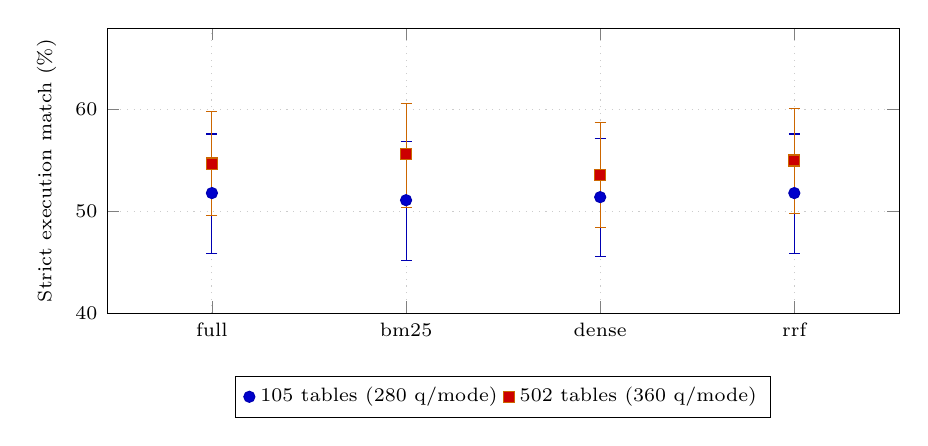
\begin{tikzpicture}
\begin{axis}[
  width=0.96\columnwidth, height=5.2cm,
  ylabel={Strict execution match (\%)},
  ymin=40, ymax=68,
  symbolic x coords={full,bm25,dense,rrf},
  xtick=data,
  enlarge x limits=0.18,
  grid=major, grid style={dotted,gray!40},
  legend style={at={(0.5,-0.22)},anchor=north,font=\scriptsize,
    legend columns=2},
  tick label style={font=\scriptsize},
  label style={font=\scriptsize},
  legend cell align=left,
]
% 105-table scale (280 questions/mode), Wilson 95% CI
\addplot+[only marks,mark=*,mark size=2pt,color=blue!70!black,
  error bars/.cd, y dir=both, y explicit,
  error bar style={color=blue!70!black}]
  coordinates {
    (full,51.8)  += (0,5.8) -= (0,5.9)
    (bm25,51.1)  += (0,5.8) -= (0,5.9)
    (dense,51.4) += (0,5.8) -= (0,5.8)
    (rrf,51.8)   += (0,5.8) -= (0,5.9)
  };
\addlegendentry{105 tables (280 q/mode)}

% 502-table scale (360 questions/mode), Wilson 95% CI
\addplot+[only marks,mark=square*,mark size=2pt,color=orange!80!black,
  error bars/.cd, y dir=both, y explicit,
  error bar style={color=orange!80!black}]
  coordinates {
    (full,54.7)  += (0,5.1) -= (0,5.1)
    (bm25,55.6)  += (0,5.0) -= (0,5.2)
    (dense,53.6) += (0,5.1) -= (0,5.2)
    (rrf,55.0)   += (0,5.1) -= (0,5.2)
  };
\addlegendentry{502 tables (360 q/mode)}
\end{axis}
\end{tikzpicture}
\caption{Two-scale retrieval ablation: strict execution match per
retrieval mode with Wilson 95\% confidence intervals
(Table~\ref{tab:ablation}). Within each scale point the intervals
overlap almost entirely and McNemar's test finds no significant
difference between any mode and the full pipeline
($p = 0.58$--$1.0$); the two scale points use different question sets
and are not comparable to each other.}
\label{fig:scale}
\end{figure}

% ──────────────────────────────────────────────────────────────
% FIGURE 3: Token Cost vs Scale
% ──────────────────────────────────────────────────────────────
\begin{figure}[!htb]
\centering
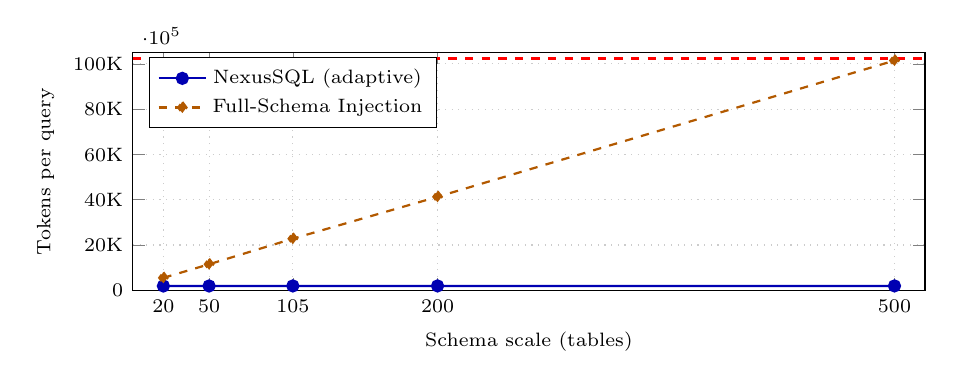
\begin{tikzpicture}
\begin{axis}[
  width=0.96\columnwidth, height=4.6cm,
  xlabel={Schema scale (tables)},
  ylabel={Tokens per query},
  xmin=0, xmax=520,
  ymin=0, ymax=105000,
  xtick={20,50,105,200,500},
  xticklabels={20,50,105,200,500},
  ytick={0,20000,40000,60000,80000,100000},
  yticklabels={0,20K,40K,60K,80K,100K},
  grid=major, grid style={dotted,gray!40},
  legend style={at={(0.02,0.98)},anchor=north west,font=\scriptsize},
  tick label style={font=\scriptsize},
  label style={font=\scriptsize},
]
% NexusSQL — flat
\addplot[color=blue!70!black,mark=*,thick,mark size=2pt]
  coordinates {(20,1900)(50,1910)(105,1932)(200,1932)(500,1932)};
\addlegendentry{NexusSQL (adaptive)}

% Full-Schema Injection — linear
\addplot[color=orange!70!black,mark=diamond*,thick,dashed,mark size=2pt]
  coordinates {(20,5500)(50,11500)(105,22800)(200,41300)(500,101500)};
\addlegendentry{Full-Schema Injection}

% Context window limit annotation
\draw[red,thick,dashed] (axis cs:0,102400) -- (axis cs:520,102400);
\node[font=\tiny,red,anchor=west] at (axis cs:5,98000) {128K ctx limit};

\end{axis}
\end{tikzpicture}
\caption{Token cost per query vs schema scale. NexusSQL's adaptive
retrieval stays constant at $\approx$1,932 tokens regardless of schema
size. Full-schema injection grows linearly, exceeding the 128K context
window limit beyond $\approx$640 tables and failing entirely.}
\label{fig:tokens}
\end{figure}

% ──────────────────────────────────────────────────────────────
% FIGURE 4: SQLAS Verdict Breakdown
% ──────────────────────────────────────────────────────────────
\begin{figure}[!htb]
\centering
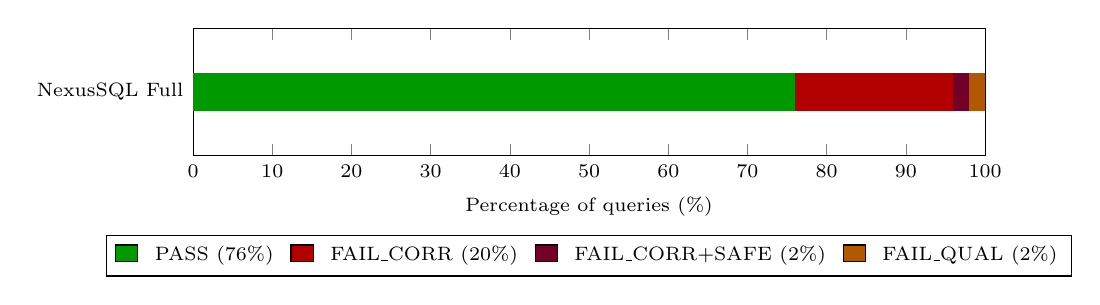
\begin{tikzpicture}
\begin{axis}[
  xbar stacked,
  width=0.96\columnwidth, height=3.2cm,
  bar width=14pt,
  xmin=0, xmax=100,
  xlabel={Percentage of queries (\%)},
  ytick={0},
  yticklabels={NexusSQL Full},
  tick label style={font=\scriptsize},
  label style={font=\scriptsize},
  legend style={at={(0.5,-0.62)},anchor=north,font=\scriptsize,
    legend columns=4, column sep=4pt},
  legend cell align=left,
]
\addplot[fill=green!60!black,draw=none]  coordinates {(76,0)};
\addlegendentry{PASS (76\%)}
\addplot[fill=red!70!black,draw=none]    coordinates {(20,0)};
\addlegendentry{FAIL\_CORR (20\%)}
\addplot[fill=purple!60!black,draw=none] coordinates {(2,0)};
\addlegendentry{FAIL\_CORR+SAFE (2\%)}
\addplot[fill=orange!70!black,draw=none] coordinates {(2,0)};
\addlegendentry{FAIL\_QUAL (2\%)}
\end{axis}
\end{tikzpicture}
\caption{SQLAS three-dimension verdict breakdown over the 100
LLM-judged queries of Table~\ref{tab:judged}. Quality and safety are
not the bottleneck (mean quality 0.889; 2/100 quality-only failures);
the dominant failure mode is incorrect SQL.}
\label{fig:verdict}
\end{figure}

% ──────────────────────────────────────────────────────────────
\section{Discussion}
\label{sec:discussion}
% ──────────────────────────────────────────────────────────────

\textbf{Token efficiency vs accuracy:}
The honest trade-off is now explicit: full-schema injection is more
accurate where the schema fits the context window (execution accuracy
0.827 on the 200-table FSI baseline), while adaptive retrieval costs
4.7\% of the tokens and is the only option once the schema exceeds the
context window. Retrieval-based schema linking should be sold to
practitioners as a cost optimization with an accuracy price, not as an
accuracy technique.

\textbf{Retrieval mode insensitivity:}
That four retrieval modes are statistically tied at both 105 and 502
tables (McNemar $p = 0.58$--$1.0$) contradicts the common expectation
that mode differences widen with scale. We hypothesize: (1) the
generator model tolerates imperfect candidate sets --- as long as the
needed tables are present, extra or reordered candidates do not change
the SQL; (2) failures are dominated by SQL-generation difficulty
(aggregation logic, multi-hop joins), which no retrieval mode fixes;
(3) Spider-derived questions are relatively simple (avg.\ 1.2 JOINs).
BEAVER benchmark queries~\cite{beaver}, sourced from real enterprise
warehouses, would better stress-test retrieval. A practical corollary:
teams can choose the cheapest retrieval infrastructure (plain BM25
requires no embedding service) without a measurable accuracy penalty
at these scales.

\subsection{Deployment Considerations}

The choice between full-schema injection and adaptive retrieval is a
cost--accuracy decision, not an accuracy--accuracy one. For databases
with $\leq 20$ tables, FSI is the pragmatically correct choice: the
token overhead is modest ($\approx$5,500 tokens), FSI is at least as
accurate, and there is no engineering overhead for maintaining
retrieval indexes.

For databases with $21$--$50$ tables, both approaches are feasible.
We recommend adaptive retrieval for cost-sensitive deployments
(83.4\% token savings) and FSI where accuracy is paramount.

For databases with $>50$ tables, the economics increasingly favor
adaptive retrieval: token savings exceed 83\% and grow with scale,
and FSI latency increases as longer prompts require more prefill time.
Organizations that can absorb the token cost may still prefer FSI for
its accuracy edge up to the point where the schema approaches the
context limit. Beyond $\approx$640 tables, FSI is technically
infeasible and adaptive retrieval is the \emph{only} viable approach.
Given the retrieval-mode tie of Section~\ref{sec:rq_ablation}, the
specific retrieval stack can be chosen on infrastructure cost alone.

\begin{table}[!htb]
\caption{Deployment Recommendations by Schema Scale}
\label{tab:deploy}
\centering
\small
\begin{tabular}{lcl}
\toprule
\textbf{Scale} & \textbf{Tables} & \textbf{Recommended approach} \\
\midrule
Small      & $\leq 20$   & Full-schema injection (FSI) \\
Medium     & 21--50      & Either; FSI for accuracy, NexusSQL for cost \\
Large      & 51--640     & NexusSQL adaptive retrieval \\
Very large & $> 640$     & NexusSQL only (FSI infeasible) \\
\bottomrule
\end{tabular}
\end{table}

\subsection{Limitations and Future Work}

Three limitations bound the current system:

\textbf{Adaptive threshold calibration.}
The 7-signal reranker thresholds were calibrated empirically on
LargeSchemaEval, which merges Spider databases. Real enterprise schemas
have different table naming conventions (e.g., \texttt{T\_VBAK},
\texttt{BKPF} in SAP naming) that may require domain-specific
calibration; our 502-table experiments still use Spider-derived
naming, so recalibration for enterprise naming conventions remains
untested.

\textbf{Human annotation study (in progress).}
SQLAS's automated verdict has not yet been validated against human
judgment; the LLM-judged PASS rate (76.0\%) is an LLM-based signal,
not a human one. A human annotation study is currently underway:
three annotators independently label approximately 100 queries using
blinded annotation sheets (annotators see the question, generated SQL,
and execution result, but not the SQLAS scores), and we will report
inter-annotator agreement (Cohen's $\kappa$, currently \humanKappa)
and the correlation between human production-readiness judgments and
the SQLAS verdict (Spearman's $\rho$, currently \humanRho). The
annotation package has been built and annotators recruited; results
will be reported in the final version of this paper. No human
correlation numbers are claimed here.

\textbf{BEAVER and Spider 2.0 evaluation.}
Our LargeSchemaEval benchmark uses merged Spider databases --- not real
enterprise data. BEAVER~\cite{beaver} provides queries over real
enterprise warehouse schemas, and Spider 2.0~\cite{spider2} introduces
real-world enterprise SQL workflows with complex multi-hop reasoning.
Both are planned evaluation targets. We expect the retrieval advantage
hypothesis (NexusSQL's FK-graph expansion matters more for complex
multi-hop queries) to be validated on these harder benchmarks.

\subsection{Threats to Validity}

\textbf{Benchmark construction bias.}
LargeSchemaEval uses merged Spider databases, which introduces prefix
confusion: BM25 must match ``\texttt{concert\_singer\_singer}'' against
the question term ``singer'', reducing term frequency overlap versus
the original single-database setting. This likely under-estimates
NexusSQL's retrieval performance on real enterprise schemas where table
names are not prefixed. The imdb anomaly (schema-only database excluded
from fair comparison) further complicates cross-scale comparisons.

\textbf{Schema scale ceiling.}
Our largest experiment is 502 tables. Real enterprise schemas (SAP:
2,000+, Oracle EBS: 1,500+) remain considerably larger, and behavior
beyond 502 tables has not been empirically verified.

\textbf{Single LLM dependency.}
All experiments use a single \texttt{gpt-5.5} deployment via Azure
OpenAI. Model-specific behaviors (instruction following, schema
grounding) may affect results --- including the retrieval-mode tie,
which could narrow or widen under a weaker generator. Evaluation with
open-source models (Llama-3, Mistral) is planned to assess retrieval
mode sensitivity across LLM backends.

\textbf{Limitations:}
(1) Adaptive threshold calibrated for single-database schemas; prefix
confusion in merged schemas degrades BM25 relevance.
(2) Full quality evaluation (faithfulness, SQL quality) requires LLM calls,
making large-scale evaluation expensive.
(3) The human correlation study is in progress; until it reports,
SQLAS's agreement with human judgment is unvalidated.

% ──────────────────────────────────────────────────────────────
\section{Conclusion}
\label{sec:conclusion}
% ──────────────────────────────────────────────────────────────

We presented SQLAS --- a multi-dimension evaluation framework for SQL
agents combining a three-dimension AND-logic verdict, a zero-LLM-call
safety suite, a schema-retrieval F1 metric, and a 15-category failure
taxonomy --- together with the LargeSchemaEval benchmark
(50/100/200/500-table scale points) and NexusSQL, a production SQL
agent used as its case study. Across the evaluation campaigns
enumerated in Table~\ref{tab:totals}, NexusSQL reaches 62.3\% execution
match on the full BIRD dev set (1,534 questions, zero-shot,
manifest-pinned), a 76.0\% PASS rate under the LLM-judged
three-dimension verdict, and 100\% read-only compliance under AST-based
enforcement.

Our key finding is a corrective one for the schema-linking literature:
in a two-scale ablation at 105 and 502 tables, four retrieval modes are
statistically indistinguishable in execution match (McNemar
$p = 0.58$--$1.0$), and full-schema injection is more accurate wherever
the schema fits the context window. Retrieval-based schema linking
earns its place as a cost optimization --- 95.3\% prompt-token
reduction at 200 tables, and the only viable architecture beyond
$\approx$640 tables --- not as an accuracy mechanism. We believe
reporting this result plainly, alongside the evaluation-integrity
methodology that surfaced it (per-row provenance, gold-set repair,
manifest pinning, full re-runs), is itself a useful contribution.

\textbf{Future work:} completing the human annotation study for SQLAS
validation; evaluation beyond 502 tables and with open-source
generators; BM25 prefix-aware documents for merged schemas; BEAVER and
Spider~2.0 enterprise benchmark evaluation.

% ──────────────────────────────────────────────────────────────
% ── AI-Generated Content Acknowledgement (required by IEEE/ICDE policy) ──
\section*{AI-Generated Content Acknowledgement}
In preparing this manuscript, the author used Claude (Anthropic, version
Sonnet 4.6) to assist with writing, editing, grammar enhancement, and
expansion of technical descriptions. All experimental results, system
design decisions, code implementation, and scientific claims are the
original work of the author. The author takes full responsibility for
the correctness and originality of the submitted content. No AI system
was used to generate experimental data, fabricate results, or produce
novel scientific contributions.

\bibliographystyle{IEEEtran}
\balance

\begin{thebibliography}{21}

\bibitem{spider}
T. Yu \textit{et al.},
``Spider: A Large-Scale Human-Labeled Dataset for Complex and
Cross-Domain Semantic Parsing and Text-to-SQL Task,''
in \textit{EMNLP}, 2018.

\bibitem{bird}
J. Li \textit{et al.},
``Can LLM Already Serve as a Database Interface? A BIg Bench for
Large-Scale Database Grounded Text-to-SQLs,''
in \textit{NeurIPS}, 2023.

\bibitem{stef}
T.~J. Arif and K. Singh,
``Agent-Agnostic Evaluation of SQL Accuracy in Production Text-to-SQL Systems,''
\textit{arXiv:2604.28049}, 2026.

\bibitem{ragas}
S. Es \textit{et al.},
``RAGAS: Automated Evaluation of Retrieval Augmented Generation,''
\textit{arXiv:2309.15217}, 2023.

\bibitem{rrf}
G.~V. Cormack, C.~L. Clarke, and S. Buettcher,
``Reciprocal Rank Fusion Outperforms Condorcet and Individual Rank
Learning Methods,''
in \textit{SIGIR}, 2009.

\bibitem{dinsql}
M. Pourreza and D. Rafiei,
``DIN-SQL: Decomposed In-Context Learning of Text-to-SQL with
Self-Correction,''
in \textit{NeurIPS}, 2023.

\bibitem{dailsql}
D. Gao \textit{et al.},
``Text-to-SQL Empowered by Large Language Models: A Benchmark Evaluation,''
\textit{arXiv:2308.15363}, 2023.

\bibitem{chess}
M. Jin \textit{et al.},
``CHESS: Contextual Harnessing for Efficient SQL Synthesis,''
\textit{arXiv:2405.16755}, 2024.

\bibitem{lostmiddle}
N.~F. Liu \textit{et al.},
``Lost in the Middle: How Language Models Use Long Contexts,''
\textit{Transactions of the ACL}, 2024.

\bibitem{beaver}
P.~B. Chen \textit{et al.},
``BEAVER: An Enterprise Benchmark for Text-to-SQL,''
\textit{arXiv:2409.02038}, 2024.

\bibitem{spider2}
F. Lei \textit{et al.},
``Spider 2.0: Evaluating Language Models on Real-World Enterprise
Text-to-SQL Workflows,''
in \textit{ICLR}, 2025.

\bibitem{ares}
J. Saad-Falcon \textit{et al.},
``ARES: An Automated Evaluation Framework for Retrieval-Augmented
Generation Systems,''
\textit{arXiv:2311.09476}, 2023.

\bibitem{trulens}
TruEra,
``TruLens: Evaluation and Tracking for LLM Experiments,''
\url{https://github.com/truera/trulens}, 2023.

\bibitem{deepeval}
Confident AI,
``DeepEval: The Open-Source LLM Evaluation Framework,''
\url{https://github.com/confident-ai/deepeval}, 2024.

\bibitem{sciencebench}
M. K{\"o}ppel \textit{et al.},
``ScienceBenchmark: A Complex Real-World Benchmark for Evaluating
Natural Language to SQL Systems,''
in \textit{VLDB}, 2024.

\bibitem{dbgpt}
T. Xue \textit{et al.},
``DB-GPT: Empowering Database Interactions with Private Large
Language Models,''
\textit{arXiv:2312.17449}, 2023.

\bibitem{ratsql}
B. Wang \textit{et al.},
``RAT-SQL: Relation-Aware Schema Encoding and Linking for Text-to-SQL
Parsers,''
in \textit{ACL}, 2020.

\bibitem{shadowgnn}
Z. Chen \textit{et al.},
``ShadowGNN: Graph Projection Neural Network for Text-to-SQL Parser,''
in \textit{NAACL}, 2021.

\bibitem{sadga}
C. Cai \textit{et al.},
``SADGA: Structure-Aware Dual Graph Aggregation Network for
Text-to-SQL,''
in \textit{NeurIPS}, 2021.

\end{thebibliography}

\end{document}
